\documentclass[a4paper,12pt,final]{article}

\usepackage[margin=1in]{geometry}
\usepackage{graphicx}
\title{
\begin{center}
  	
\includegraphics[scale=0.3]{101Logo.png} 
  \end{center}
  \textbf{\\}
CSIR - Distributed Application Manager\\
Functional Requirements and Design Document\\
}
\author{101 Solutions}

\begin{document}
\maketitle
\begin{center}
Version 0.9
\end{center}
\textbf{\\}
\textbf{\\}
\textbf{\\}
\textbf{\\}
\textbf{\\}
\textbf{\\}
\begin{center}
\begin{tabular}{|l|l|}
\hline
Francois Germishuizen & 11093618\\
\hline
Jaco Swanepoel & 11016354\\
\hline
Henko van Koesveld & 11009315\\
\hline
\end{tabular}
\end{center}
\thispagestyle{empty}
\newpage
\thispagestyle{empty}
\textbf{\large{Change Log}}
\vspace{6pt}\newline
\begin{tabular}{|l|l|l|}
\hline
Date & Version & Description\\
\hline
13 Sept & Version 0.1 & Document Created\\
\hline
13 Sept & Version 0.2 & Added usecase diagrams\\
\hline
13 Sept & Version 0.3 & Added AddBuild, RequestSysInfo and GetSysInfo usecase\\
\hline
13 Sept & Version 0.4 & Added Upcoming usecases and Simulations\\
\hline
13 Sept & Version 0.5 & Added overall processes and adjusted margins\\
\hline
13 Sept & Version 0.6 & Added AddSlave, StartServer, StopServer and SetPort usecase\\
\hline
13 Sept & Version 0.7 & Added Glossary\\
\hline
13 Sept & Version 0.8 & Added Class diagrams\\
\hline
13 Sept & Version 0.9 & Added AddBuild via network usecase\\
\hline
\end{tabular}
\newpage
\tableofcontents
\thispagestyle{empty}
\newpage

\pagenumbering{arabic}
\section{Overview}
\subsection{Background}
The CSIR is actively developing a distributed simulation framework that ties
in with various other real systems and is used to exchange information
between them. The client has a number of configurations of this system
depending on the requirements of the client which can involve various
external applications as well.\\
\textbf{\\}
One of the issues the client has is to quickly distribute the latest build or
configuration files of their software over various computers that are needed
for an experiment. In some cases the same computers may be used for other
experiments which mean each of the computers may need to have various
builds and configuration options.\\
\textbf{\\}
Another issue they experience is the running, stopping and restarting of
the complete simulation. During a simulation it may be determined that
certain configuration options may need to be changed and distributed to the
affected machines, in which case either all or some components will need to
be restarted which can become tedious and time consuming.
\subsection{Business opportunity}
The goal of our project is to develop an application which is able to maintain
various build versions of the simulation framework and distribute these builds
to certain designated machines that may be required for an experiment. The
application will monitor system statistics of the various machines attached
to an experiment and will have the ability to execute applications on those
machines which will have different configuration options.\\
\textbf{\\}
The application will consist of a master and slave component where the
master is used to control the distribution of slaves. From the master one will
be able to start an experiment which will run the relevant applications on all
the necessary machines.




\newpage
\section{Use Cases}
We have both a master and slave application. The master is called AppMan and the slave is called AppManClient.\\
\textbf{\\}
Below is a use case of the AppMan system as it currently is:\\
\begin{center}
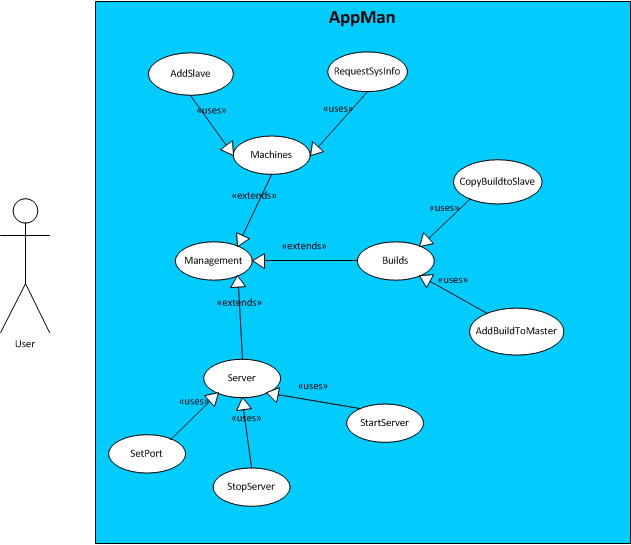
\includegraphics[scale=0.8]{UseCaseAppMan.png}
\end{center}
Below is a use case diagram of the AppManClient system as it currently is:\\
\begin{center}
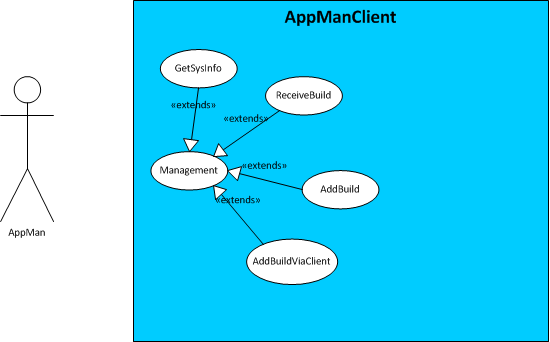
\includegraphics[scale=0.7]{UseCaseAppManClient.png}
\end{center}


\subsection{AddBuild usecase}
The following activity diagram is applicable to both AddBuildToMaster in AppMan as well as AddBuildViaClient in AppManClient.\\
\textbf{\\}
\begin{center}
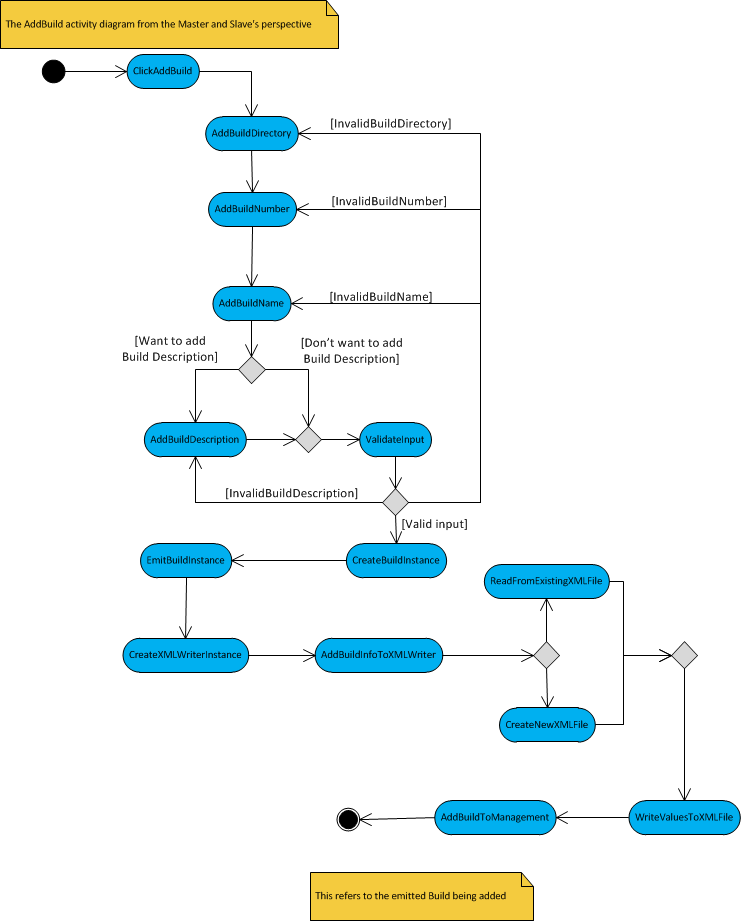
\includegraphics[scale=0.8]{AddBuildActivity.png}
\end{center}


\subsection{RequestSysInfo usecase}
The following activity diagram is applicable to the RequestSysInfo usecase in AppMan.\\
\textbf{\\}
\begin{center}
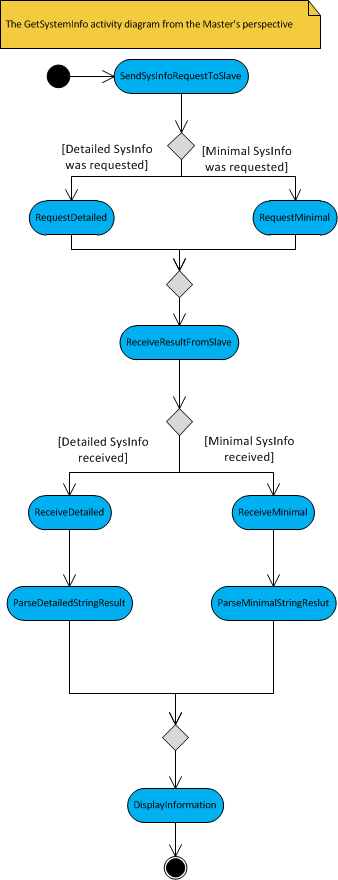
\includegraphics[scale=0.95]{GetSystemInfoActivityMASTER.png}
\end{center}


\subsection{GetSysInfo usecase}
The following activity diagram is applicable to the GetSysInfo usecase in AppManClient.\\
\textbf{\\}
\begin{center}
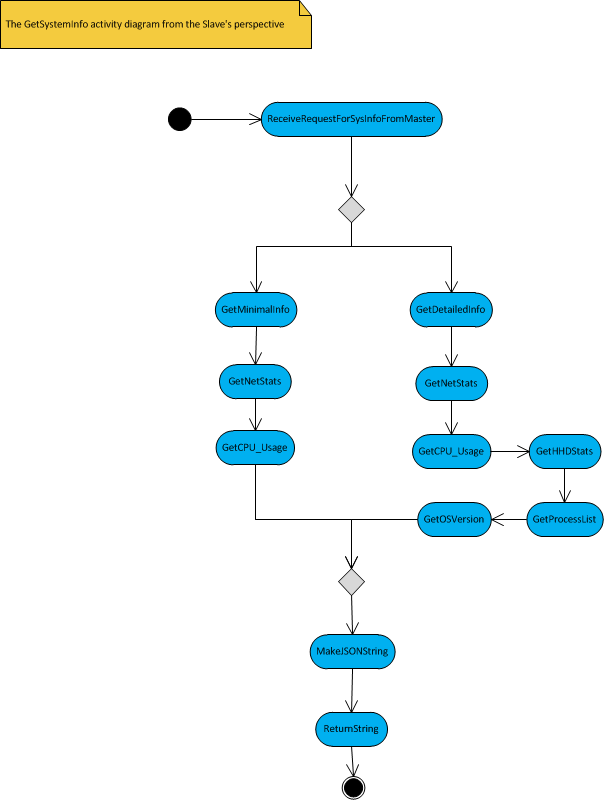
\includegraphics[scale=1]{GetSystemInfoActivitySLAVE.png}
\end{center}




\subsection{AddSlave usecase}
The following activity diagram is applicable to the AddSlave usecase in AppMan.\\
\textbf{\\}
\begin{center}
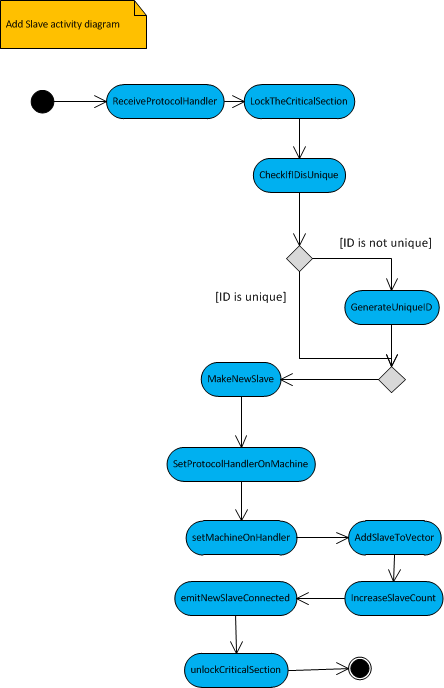
\includegraphics[scale=1]{AddSlaveActivity.png}
\end{center}



\newpage
\subsection{AddBuild via network usecase}
The following activity diagram is applicable to the AddBuild usecase in AppManClient.\\
\textbf{\\}
\begin{center}
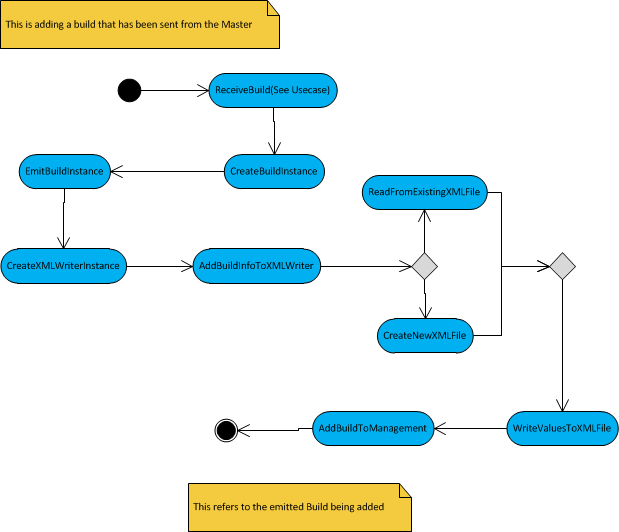
\includegraphics[scale=1]{AddBuildSlaveActivity.png}
\end{center}



\newpage
\subsection{StartServer usecase}
The following activity diagram is applicable to the StartServer usecase in AppMan.\\
\textbf{\\}
\begin{center}
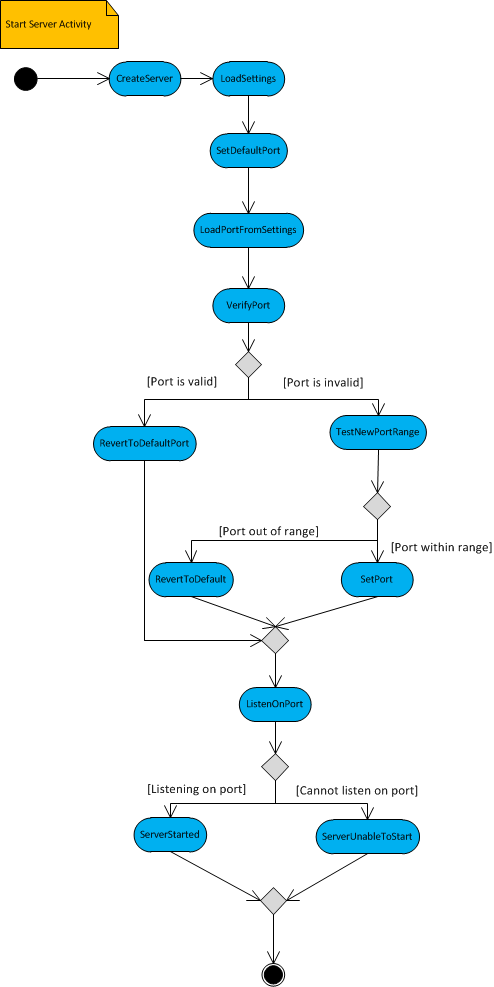
\includegraphics[scale=0.8]{StartServer.png}
\end{center}




\newpage
\subsection{SetPort usecase}
The following activity diagram is applicable to the SetPort usecase in AppMan.\\
\textbf{\\}
\begin{center}
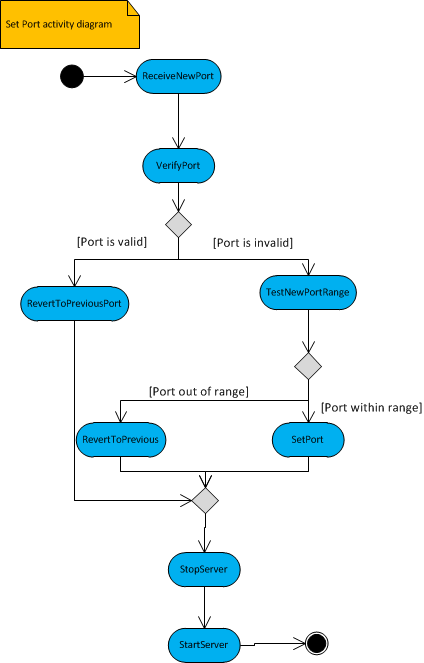
\includegraphics[scale=1]{SetPort.png}
\end{center}




\newpage
\subsection{StopServer usecase}
The following activity diagram is applicable to the StopServer usecase in AppMan.\\
\textbf{\\}
\begin{center}
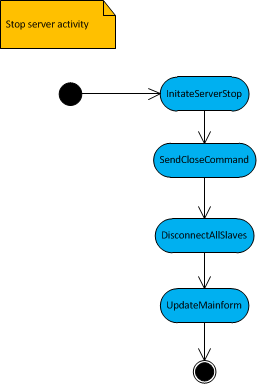
\includegraphics[scale=1]{StopServer.png}
\end{center}










\newpage
\section{Upcoming usecases}
This section is for the documentation of soon to be implemented usecases.


\subsection{Simulations}
Simulations are a set of builds to be run in specific order on a set of slaves.

\subsubsection{AddSimulation}
A simulation must be added to AppMan in the following way:
\begin{center}

\includegraphics[scale=0.9]{AddSimulationActivity.png}
\end{center}

\subsubsection{RunSimulation AppMan}
A simulation is run from AppMan in the following way:
\begin{center}
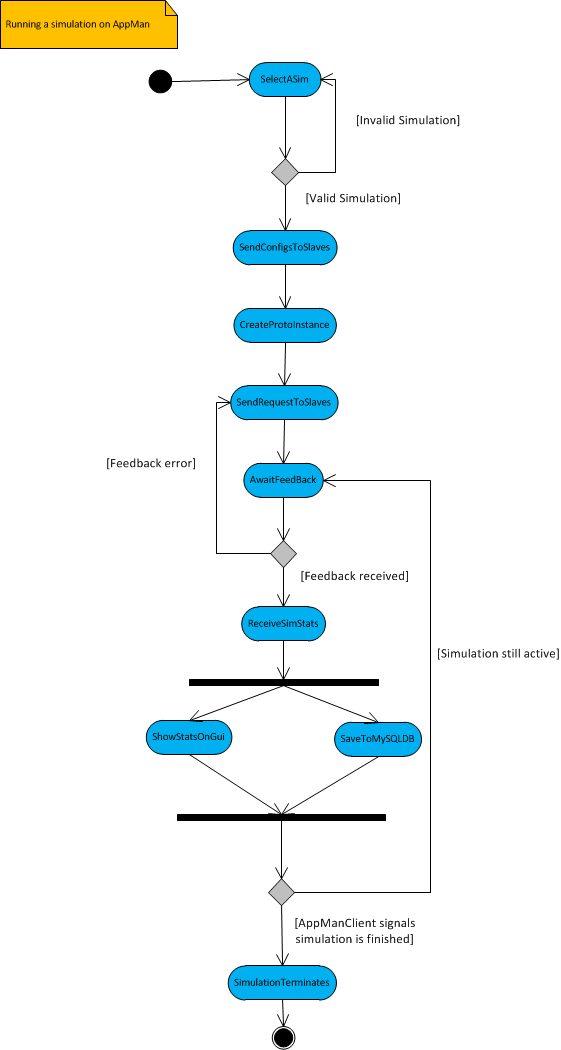
\includegraphics[scale=0.8]{RunningASimOnAppMan.png}
\end{center}

\subsubsection{RunSimulation AppManClient}
A simulation is run from AppManClient in the following way:
\begin{center}
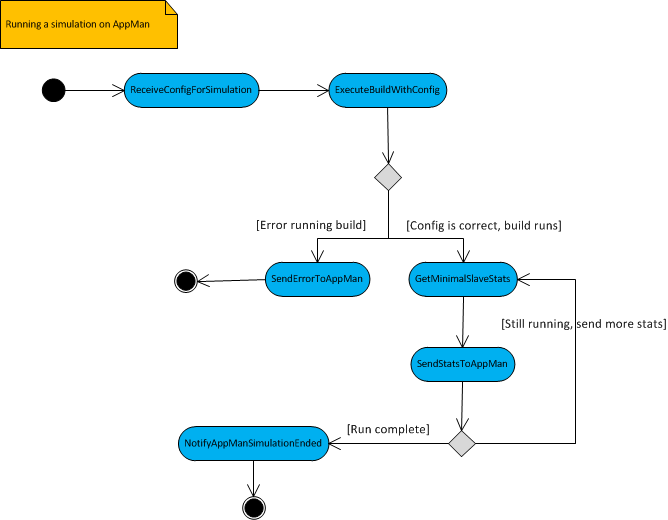
\includegraphics[scale=0.9]{RunningASimOnAppManClient.png}
\end{center}



\newpage
\section{Class diagrams}
\subsection{AppMan Class Diagram}
Due to its large size, the class diagram is split into multiple, seperate diagrams. Classes will be repeated to show how they all link.\\
\begin{center}
	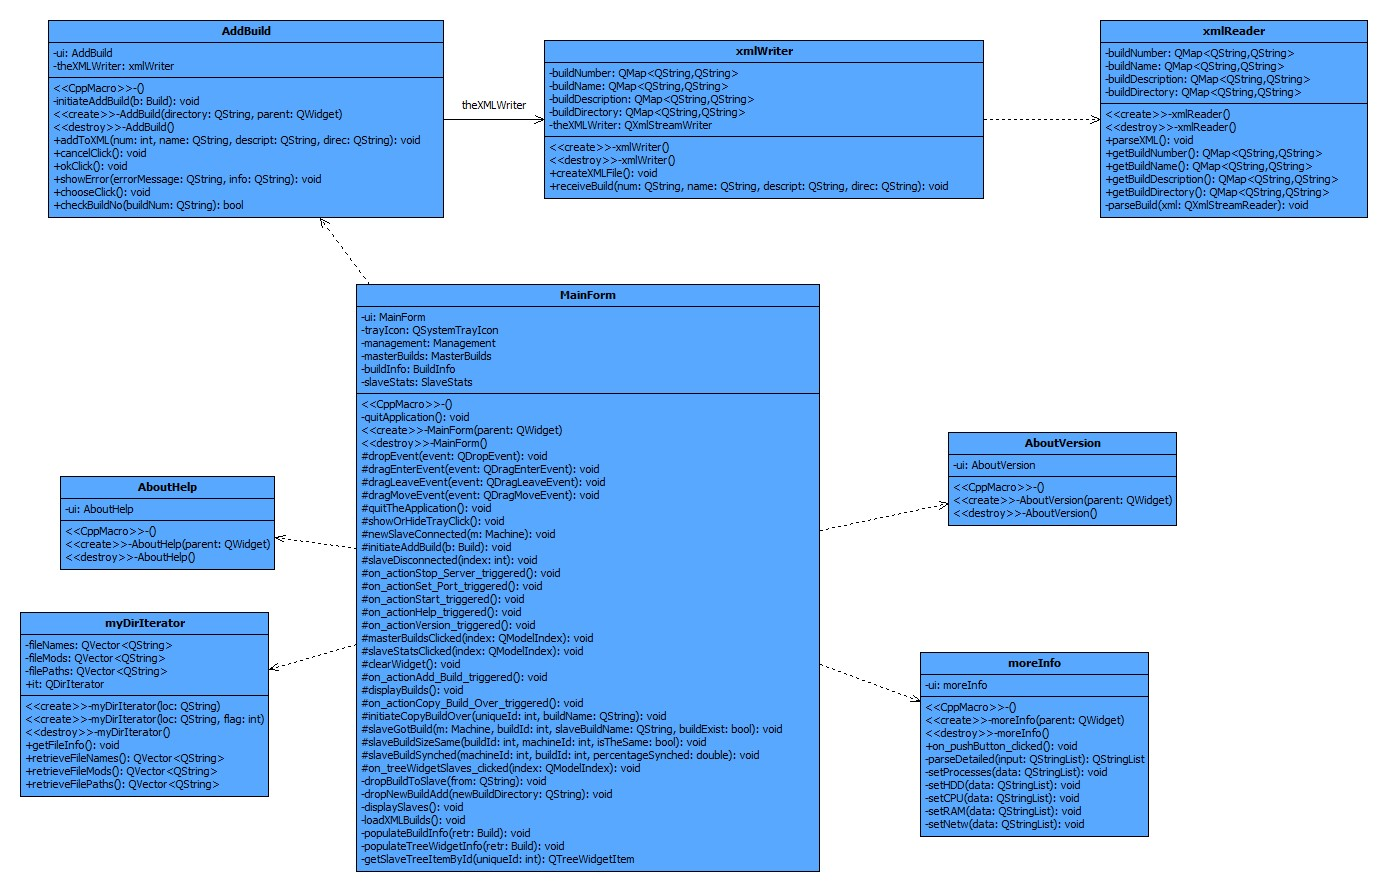
\includegraphics[angle = 90,scale = 0.42]{MainformNew.jpg}
\end{center}
\begin{center}
	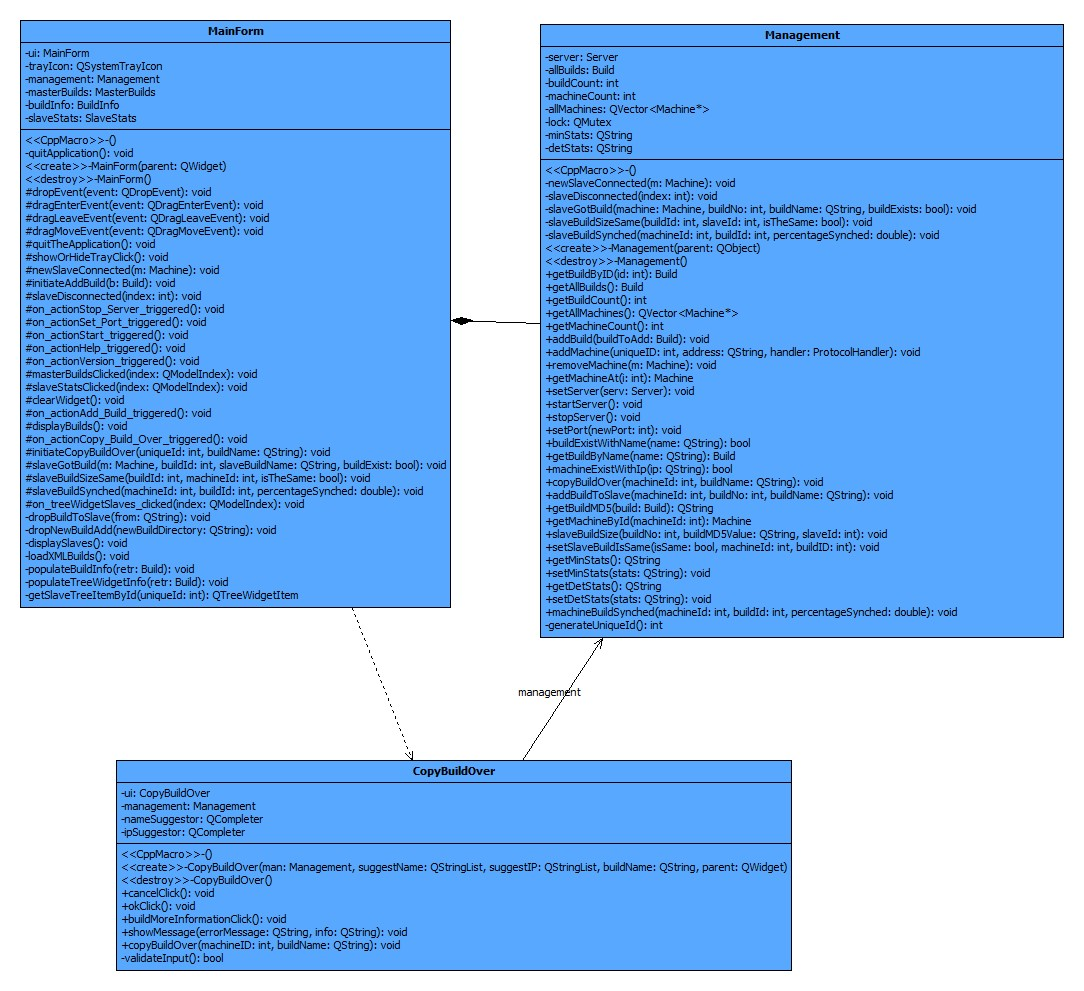
\includegraphics[angle = 90,scale = 0.5]{Mainformnew2.jpg}
\end{center}
\begin{center}
	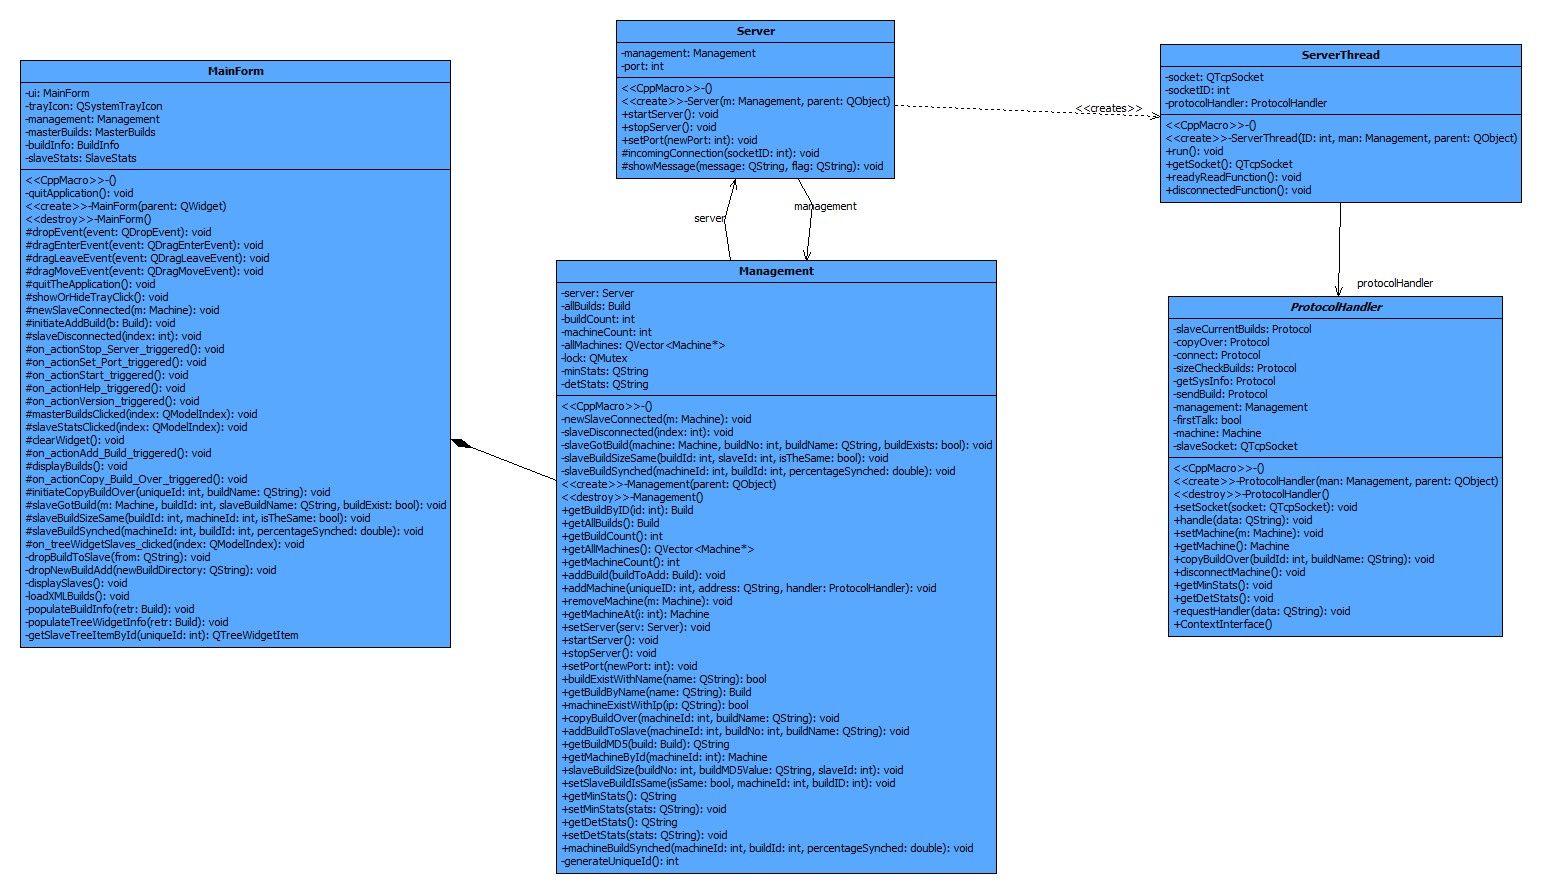
\includegraphics[angle = 90,scale = 0.45]{Server.jpg}
\end{center}
\begin{center}
	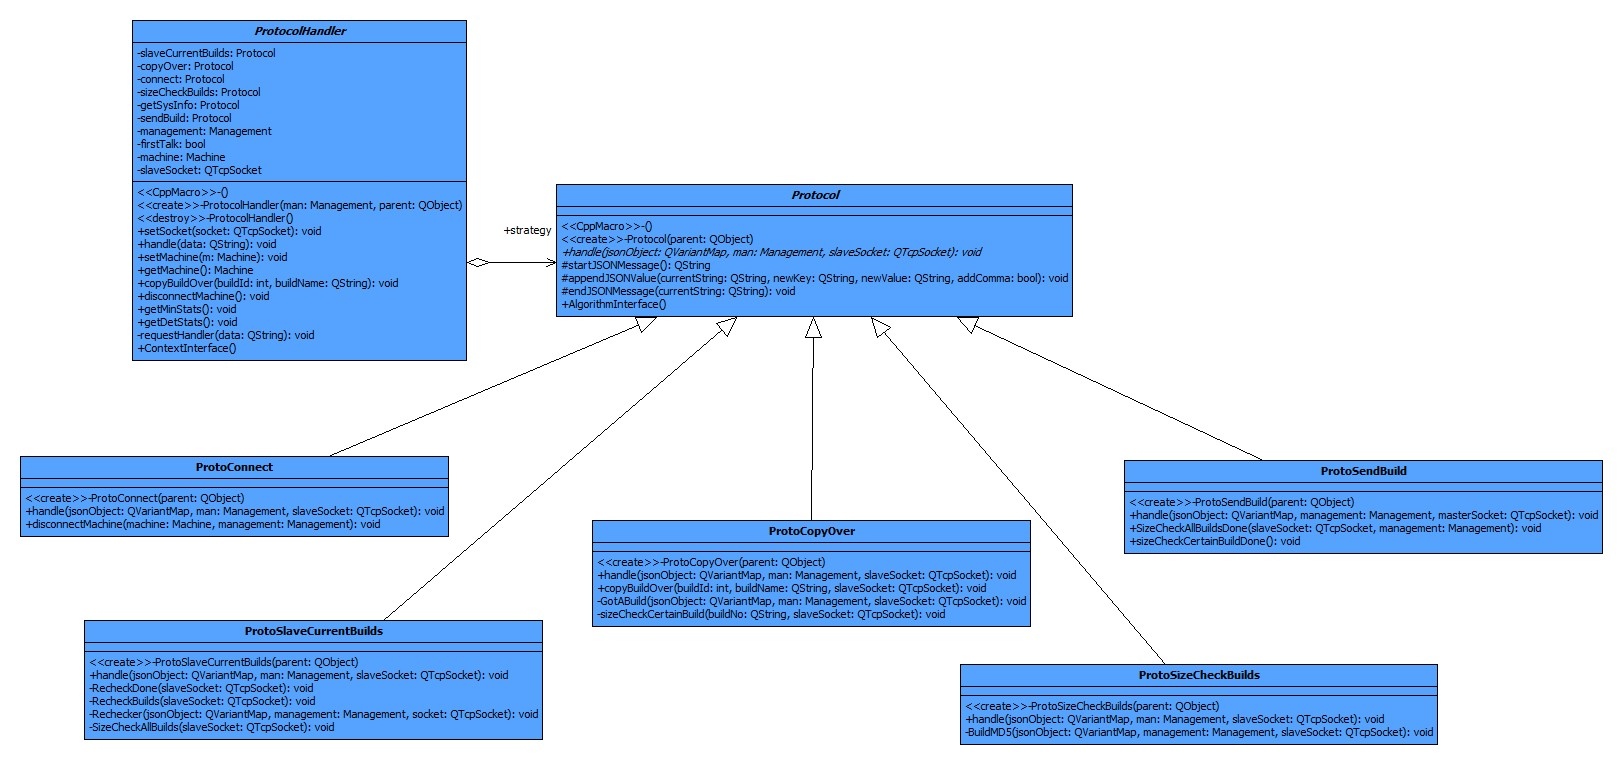
\includegraphics[angle = 90,scale = 0.45]{Protocols.jpg}
\end{center}
\begin{center}
	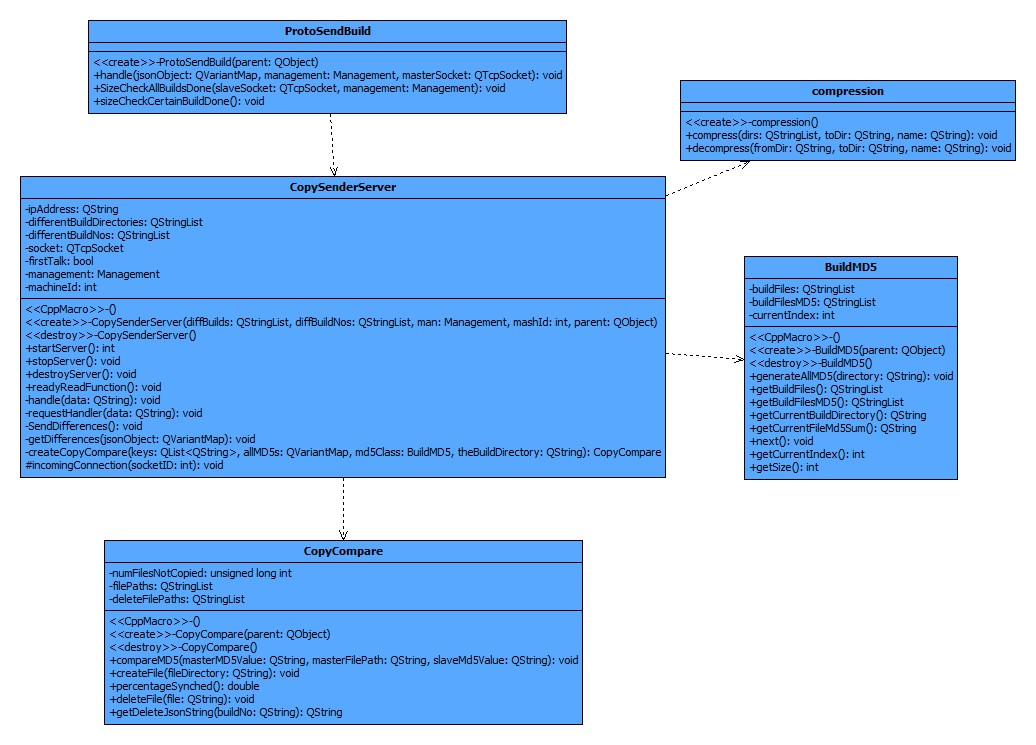
\includegraphics[angle = 90,scale = 0.65]{BuildCopy.jpg}
\end{center}
\begin{center}
	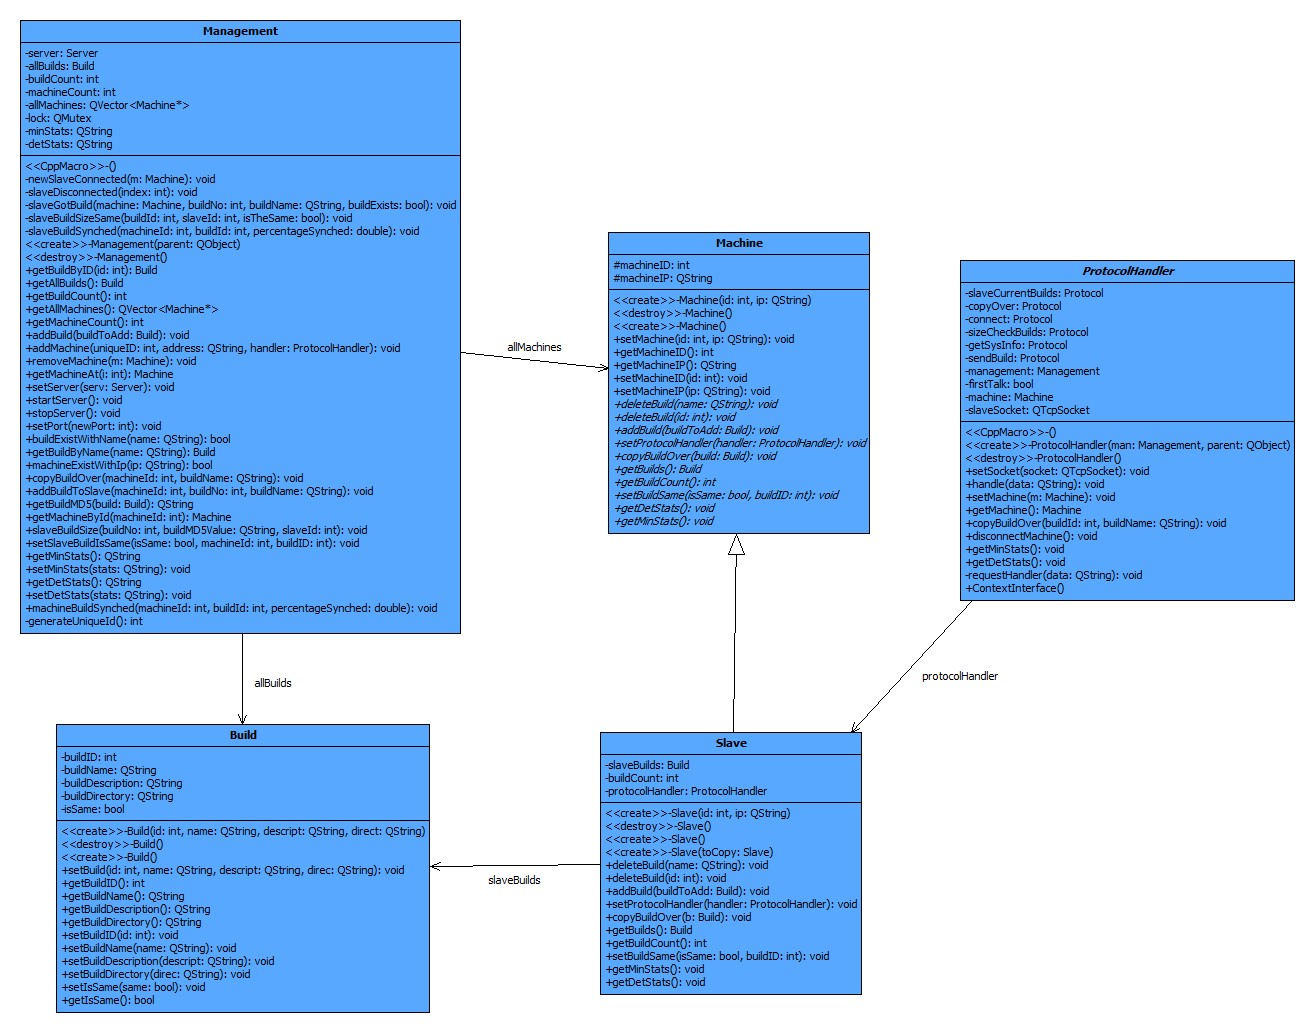
\includegraphics[angle = 90,scale = 0.47]{Slave.jpg}
\end{center}
\newpage
\subsection{AppManClient Class Diagram}
Due to its large size, the class diagram is split into multiple, seperate diagrams. Classes will be repeated to show how they all link.\\
\begin{center}
	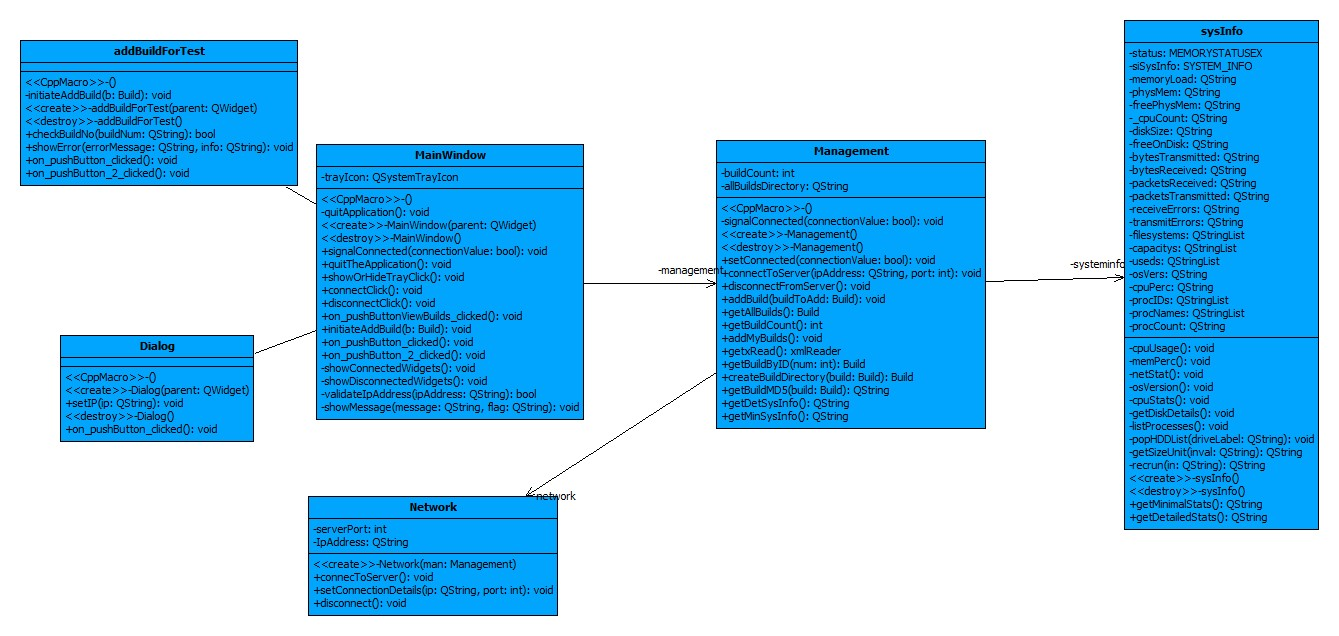
\includegraphics[angle = 90,scale = 0.47]{Part1.jpg}
\end{center}
\begin{center}
	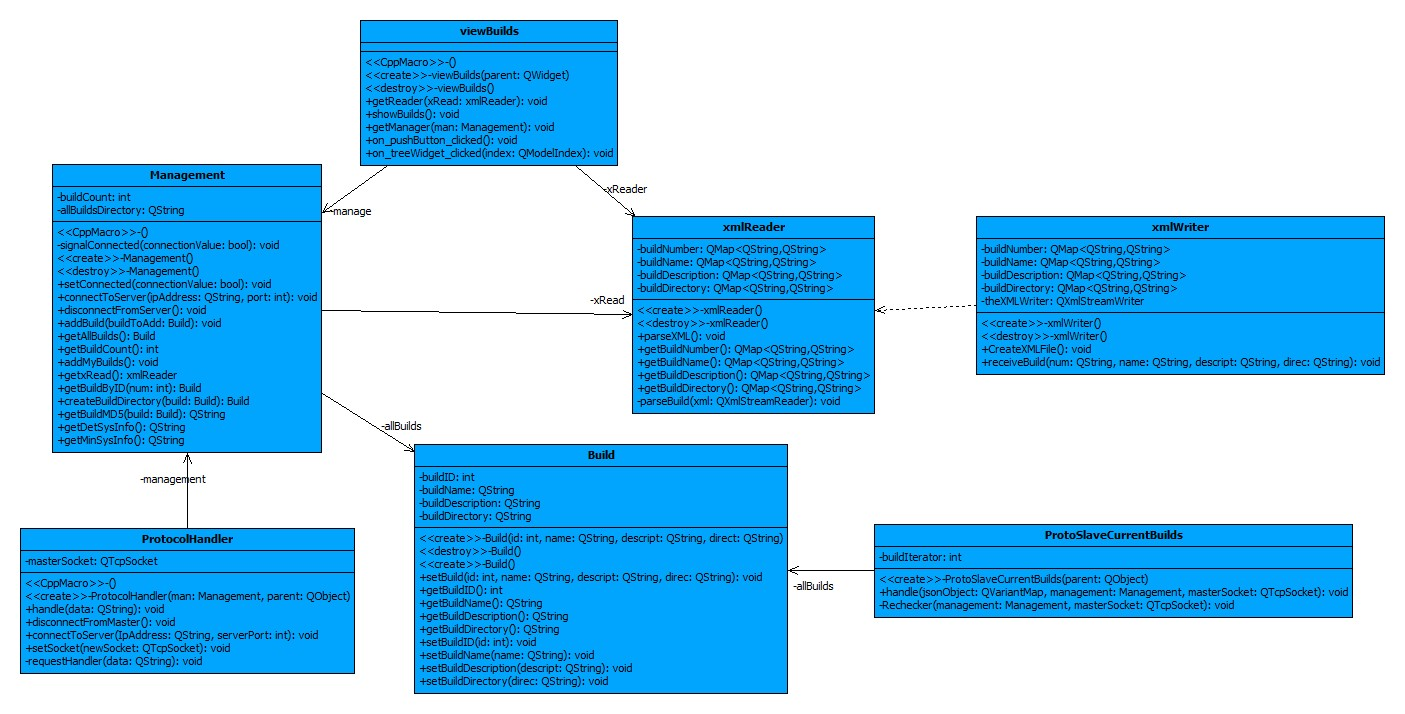
\includegraphics[angle = 90,scale = 0.47]{Part1_1.jpg}
\end{center}
\begin{center}
	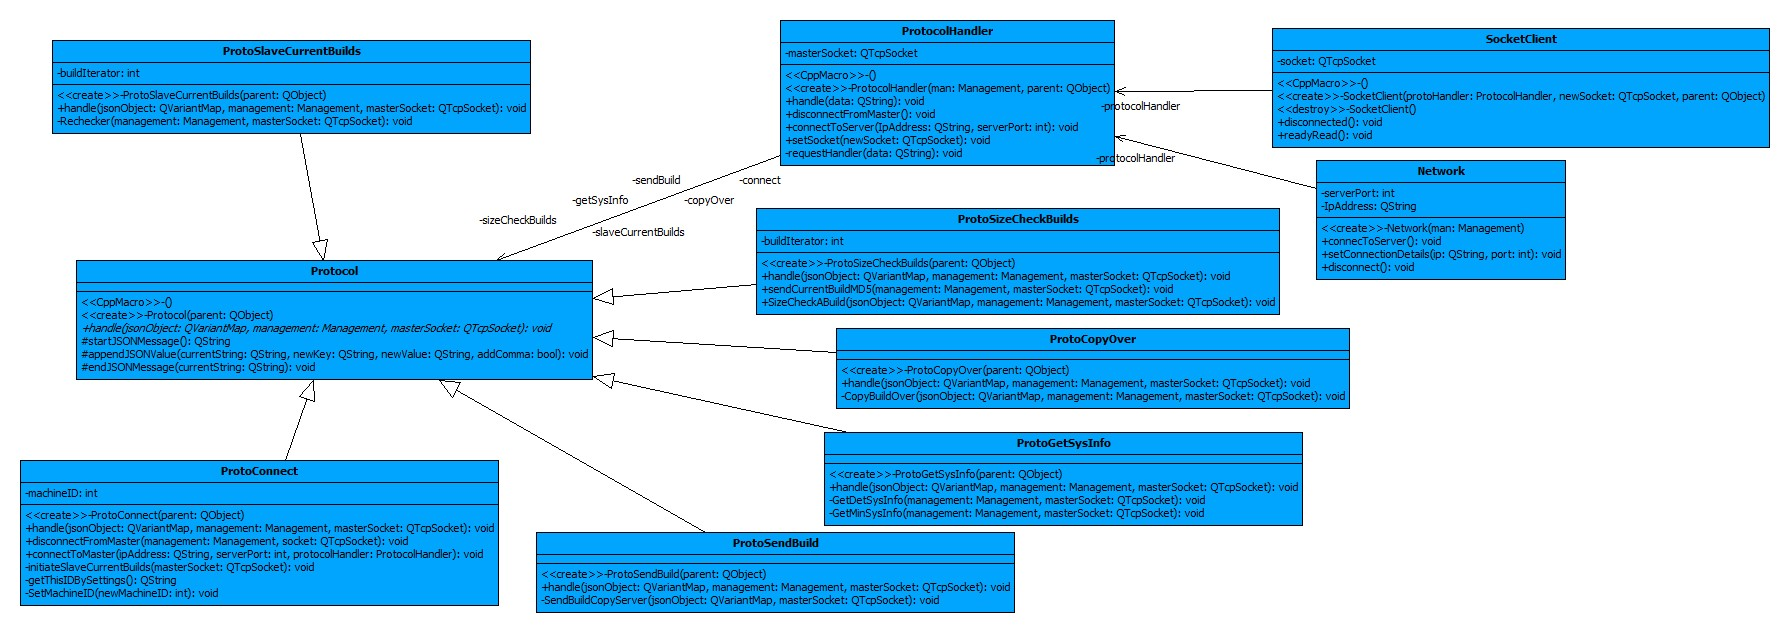
\includegraphics[angle = 90,scale = 0.4]{Part2.jpg}
\end{center}
\begin{center}
	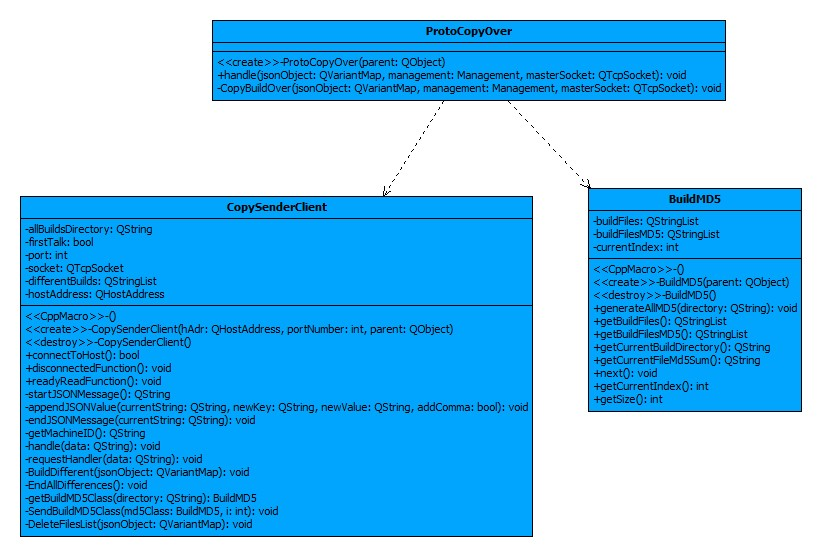
\includegraphics[angle = 90,scale = 0.7]{Part3.jpg}
\end{center}


\newpage
\section{Overall Processes}
This section is for the Activity diagrams based on current progress of AppMan and AppManClient respectively.
\subsection{AppMan}
\begin{center}
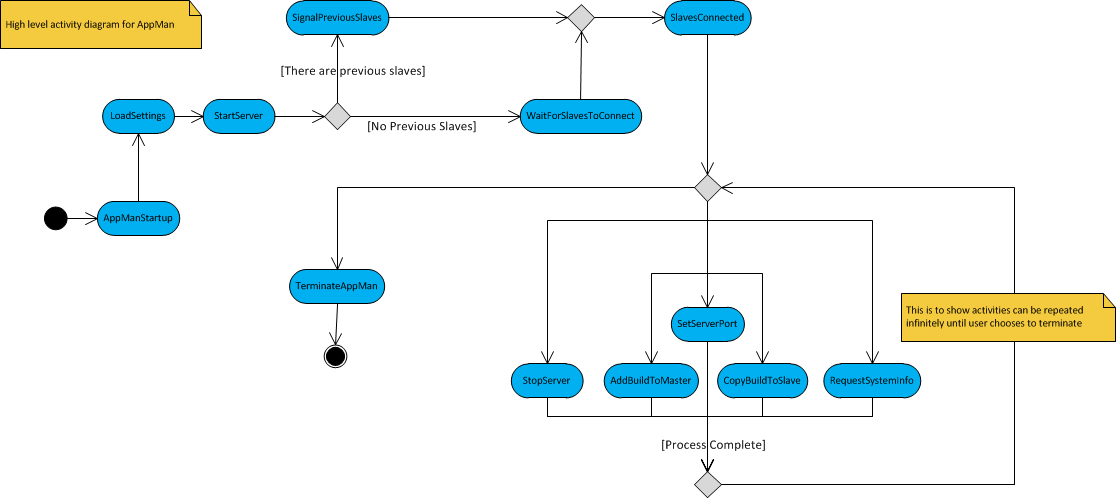
\includegraphics[angle = 90, scale=0.7]{MasterMainActivity.png}
\end{center}
\newpage
\subsection{AppManClient}
\begin{center}
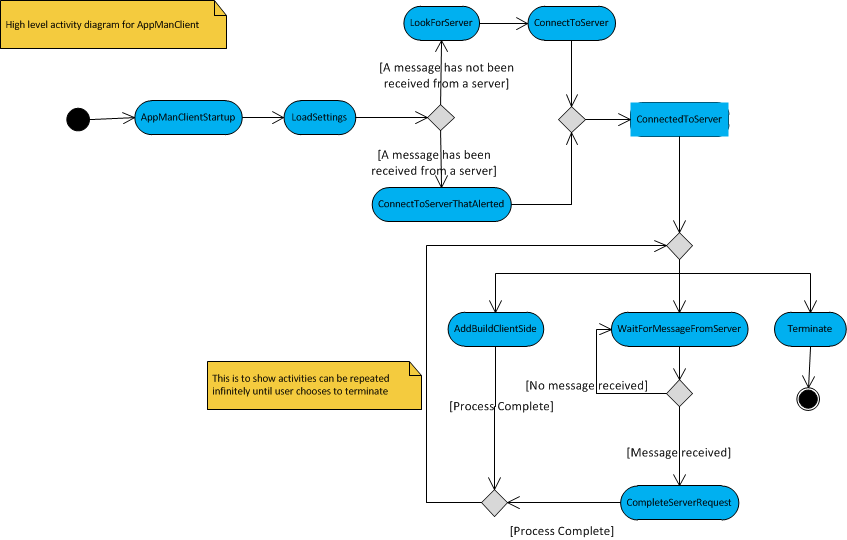
\includegraphics[angle = 90, scale=1]{SlaveMainActivity.png}
\end{center}



\newpage
\section{Communication Protocol}





\newpage
\section{Glossary}
\begin{itemize}
\item{Build - An application build version that could potentially be distributed to slave computers.}
\item{Slave - A computer that will be controlled via a master computer. Application builds will be sent to this computer.}
\item{Master - A computer that will control Slaves across a network.}
\item{Server - A machine waiting on the network for connections from other machines.}
\item{GUI - Graphical User Interface with which a user can control the project.}
\item{Project - This project. The distributed application manager.}
\item{Application Configuration - Environment variables that are specified when running an application.}
\end{itemize}




\end{document}